\documentclass[12pt]{mwart}\usepackage[]{graphicx}\usepackage[]{xcolor}
% maxwidth is the original width if it is less than linewidth
% otherwise use linewidth (to make sure the graphics do not exceed the margin)
\makeatletter
\def\maxwidth{ %
  \ifdim\Gin@nat@width>\linewidth
    \linewidth
  \else
    \Gin@nat@width
  \fi
}
\makeatother

\definecolor{fgcolor}{rgb}{0.345, 0.345, 0.345}
\newcommand{\hlnum}[1]{\textcolor[rgb]{0.686,0.059,0.569}{#1}}%
\newcommand{\hlstr}[1]{\textcolor[rgb]{0.192,0.494,0.8}{#1}}%
\newcommand{\hlcom}[1]{\textcolor[rgb]{0.678,0.584,0.686}{\textit{#1}}}%
\newcommand{\hlopt}[1]{\textcolor[rgb]{0,0,0}{#1}}%
\newcommand{\hlstd}[1]{\textcolor[rgb]{0.345,0.345,0.345}{#1}}%
\newcommand{\hlkwa}[1]{\textcolor[rgb]{0.161,0.373,0.58}{\textbf{#1}}}%
\newcommand{\hlkwb}[1]{\textcolor[rgb]{0.69,0.353,0.396}{#1}}%
\newcommand{\hlkwc}[1]{\textcolor[rgb]{0.333,0.667,0.333}{#1}}%
\newcommand{\hlkwd}[1]{\textcolor[rgb]{0.737,0.353,0.396}{\textbf{#1}}}%
\let\hlipl\hlkwb

\usepackage{framed}
\makeatletter
\newenvironment{kframe}{%
 \def\at@end@of@kframe{}%
 \ifinner\ifhmode%
  \def\at@end@of@kframe{\end{minipage}}%
  \begin{minipage}{\columnwidth}%
 \fi\fi%
 \def\FrameCommand##1{\hskip\@totalleftmargin \hskip-\fboxsep
 \colorbox{shadecolor}{##1}\hskip-\fboxsep
     % There is no \\@totalrightmargin, so:
     \hskip-\linewidth \hskip-\@totalleftmargin \hskip\columnwidth}%
 \MakeFramed {\advance\hsize-\width
   \@totalleftmargin\z@ \linewidth\hsize
   \@setminipage}}%
 {\par\unskip\endMakeFramed%
 \at@end@of@kframe}
\makeatother

\definecolor{shadecolor}{rgb}{.97, .97, .97}
\definecolor{messagecolor}{rgb}{0, 0, 0}
\definecolor{warningcolor}{rgb}{1, 0, 1}
\definecolor{errorcolor}{rgb}{1, 0, 0}
\newenvironment{knitrout}{}{} % an empty environment to be redefined in TeX

\usepackage{alltt} %mwart, mwrep, mwbk
\usepackage[utf8]{inputenc} % kodowanie
\usepackage{polski}
\usepackage{graphicx}
\linespread{1.3}
\usepackage{mathtools, amsmath, amssymb} % pakiety do wzorów
\usepackage{icomma} % przecinek pomiędzy liczbami bez odstępu
\usepackage{tabularx}
\usepackage{listings}

\lstset{
    language=C,
    basicstyle=\ttfamily\small,
    keywordstyle=\color{blue}\bfseries,
    commentstyle=\color{green!50!black},
    morekeywords={function, int, return, if, for, mod, xor},
    tabsize=4,
    frame=single,
    breaklines=true,
    showstringspaces=false,
}
\mathtoolsset{showonlyrefs}

\author{Roksana Krysztofiak}
\title{Wprowadzenie do symulacji i metod Monte Carlo - projekt 1}
\IfFileExists{upquote.sty}{\usepackage{upquote}}{}
\begin{document}
\maketitle

\section*{Cel projektu}
W naszym projekcie chcemy sprawdzić jakość różnych generatorów liczb pseudolosowych oraz porównać je za pomocą różnych testów statystycznych.

\section*{Generatory}
Użyjemy 4 różnych generatorów w celu otrzymania liczb pseudolosowych. W tym projekcie wybrałam RC4(32), LCG, GLCG, BBSG oraz MT. Ostatnie dwa nie były opisywane w treści naszego zadania, zatem zrobimy to teraz.

\subsection*{BBSG}
Blum-Blum-Shub (BBSG) to generator liczb pseudolosowych, którego działanie opiera się na trudności rozkładu dużych liczb na czynniki pierwsze. Algorytm dla tego generatora, gdy generujemy pseudolosową sekwencję bitów $z_1, z_2, ..., z_l$ długośli $l$:
\begin{itemize}
  \item Wybieramy dwie duże liczby pierwsze $p$ i $q$, które dają resztę 3 w działaniu modulo 4. Następnie obliczamy $n = p \cdot q$

  \item Wybieramy ziarno początkowe $x_0$, które jest liczbą całkowitą z przedziału [1, n-1] oraz względnie pierwsze z n
  \item Dla i od 1 do l: \newline
    a) $x_i <- x_{i-1}^2 mod n$ \newline
    b) $z_i <-$ najmniej znaczący bit z $x_i$
  \item Wynikiem jest sekwencja $z_1, z_2, ..., z_l.$
    
\end{itemize}
\subsection*{MT}
Mersenne Twister, to bardzo popularny generator liczb pseudolosowych, wykorzystywany m.in. w Pythonie w funkcji random.random z modułu random. Ma on bardzo długi okres wynoszący $2^{19937}-1$. 
Poniżej znajduje się implementacja algorytmu Mersenne Twister w pseudokodzie:

\begin{lstlisting}
// Utworz tablice 624 elementow do przechowywania 
//stanu generatora
int[0..623] MT
int index = 0

// Inicjuj generator przy uzyciu ziarna
function initializeGenerator(int seed) {
    MT[0] := seed
    for i from 1 to 623 {
        MT[i] := last 32 bits of(1812433253 * (MT[i-1] 
          xor (right shift by 30 bits(MT[i-1]))) + i) 
    }
}

// Utworz pseudolosowa liczbe na podstawie indeksu,
// wywolaj generateNumbers() aby utworzyc nowa tablice 
//pomocnicza co 624 liczby
function extractNumber() {
    if index == 0 {
        generateNumbers()
    }
    
    int y := MT[index]
    y := y xor (right shift by 11 bits(y))
    y := y xor (left shift by 7 bits(y) and (2636928640)) 
    y := y xor (left shift by 15 bits(y) and(4022730752)) 
    y := y xor (right shift by 18 bits(y))
    
    index := (index + 1) mod 624
    return y
}

// Generuj tablice 624 liczb
function generateNumbers() {
    for i from 0 to 623 {
        int y := 32nd bit of(MT[i]) + last 31 
          bits of(MT[(i+1) mod 624])
        MT[i] := MT[(i + 397) mod 624] xor 
          (right shift by 1 bit(y))
        if (y mod 2) == 1 { 
            MT[i] := MT[i] xor (2567483615)
        }
    }
}
\end{lstlisting}

\section*{Testy}
W celu sprawdzenia jakości generatorów przyjrzymy się p$\_$wartością różnych testów. Tutaj wykorzystałam testy Kołomogorowa-Smirnowa(KS), \newline chi-kwadrat(CHI2) oraz Cramera-von Misesa(CVM). 

\subsection*{CVM}
Test Cramera–von Misesa(CVM) jest statystycznym testem zgodności używanym do sprawdzenia, czy dane pochodzą z określonego rozkładu. Jest oparty na kwadratowej odległości między empiryczną dystrybuantą \( F_n(x) \) a teoretyczną dystrybuantą \( F(x) \).

Statystyka testu jest zdefiniowana jako:
\[
W^2 = n \int_{-\infty}^\infty \left( F_n(x) - F(x) \right)^2 \, dF(x),
\]
gdzie \( n \) to liczba obserwacji, \( F_n(x) \) jest empiryczną dystrybuantą danych, a \( F(x) \) to teoretyczna dystrybuanta.

\newpage
\section*{Wyniki i wnioski}
Na początku poprzez każdy generator stworzyliśmy 1000 liczb. Następnie poddaliśmy je naszym testom w celu otrzymania p$\_$wartości. Z powodu, że przy prawdziwej hipotezie zerowej rozkład p$\_$wartości powinien mieć rozkład jednostajny na przedziale$(0,1)$, powtarzamy ten eksperyment więcej razy i wyniki przedstawiamy na wykresie poniżej. W tym przypadku obliczenia powtarzaliśmy $2^{15}$ razy.

\begin{center}
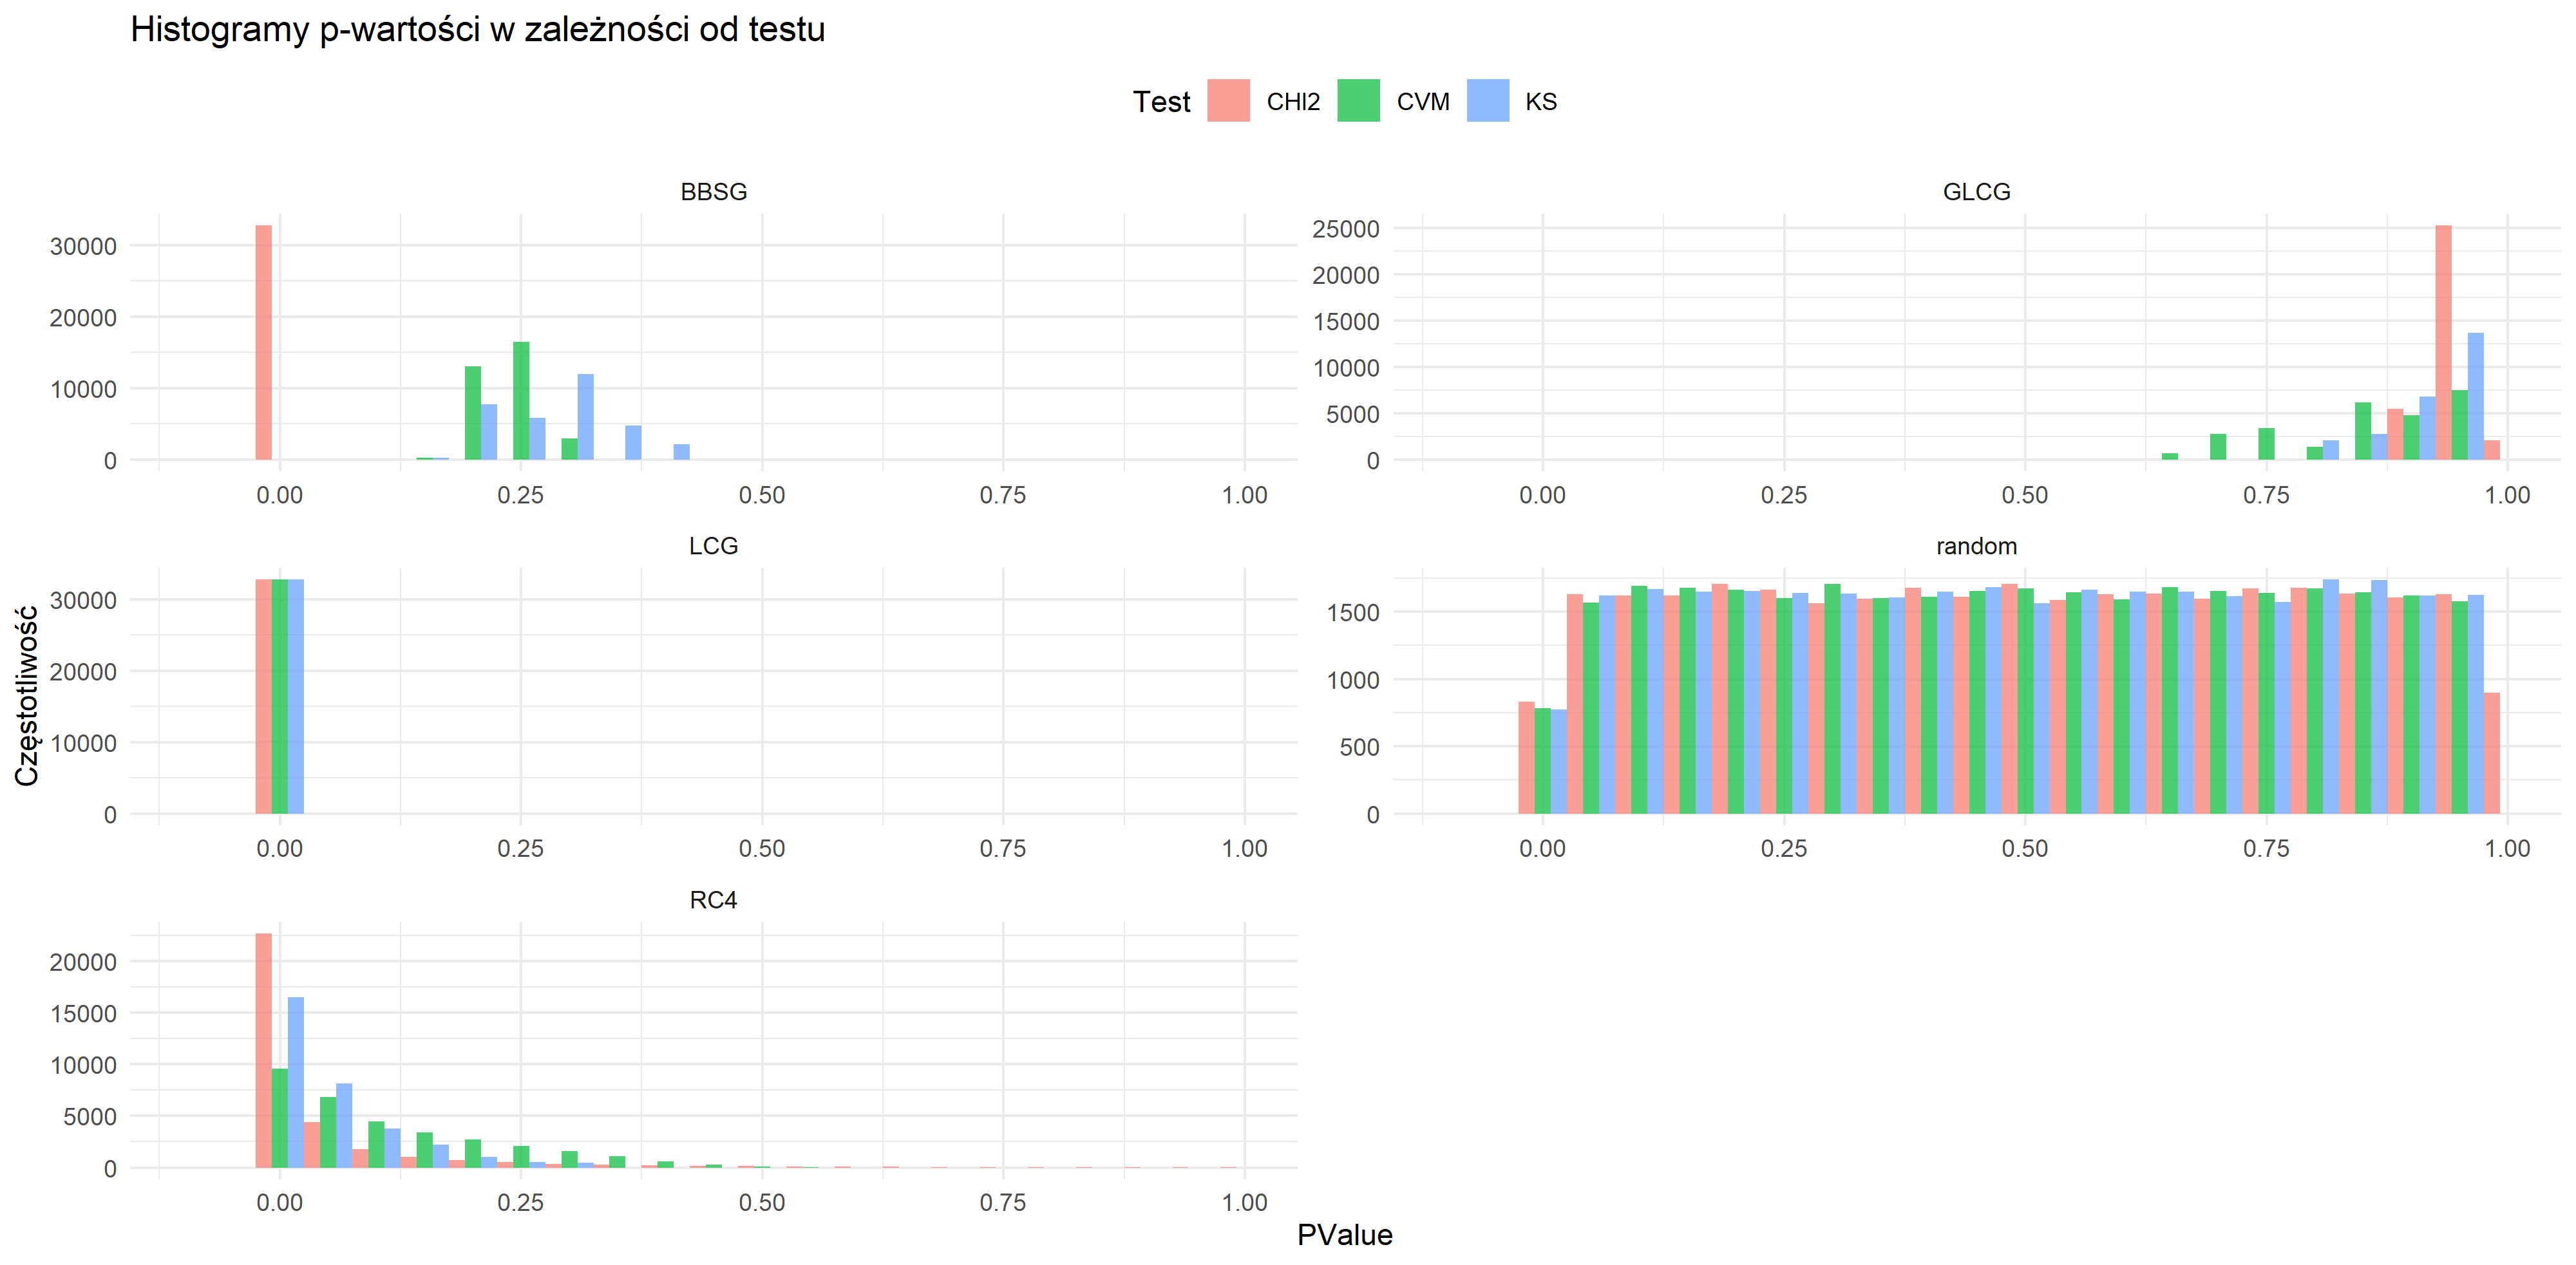
\includegraphics[scale=0.45]{p_wartosc_a_test.png}
\caption{Wyk.1 Rozkład p wartości testów dla  wygenerowanych ciagów liczb długości 1000}
\end{center}


Widzimy, że rozkład p$\_$wartości dla generatora Mersenne Twistera najbardziej przybliża rozkład jednostajny. Jest on najlepszym ze wszytkich opisanych tu generatorów. Co ciekawe, wysokie wartości dla GLCG mogłyby sugerować, że jest on dobrym generatorem, natomiast rozkład tych p$\_$wartości już nie. Warto zauważyć, że dla BBSG dla testu chi-kwadrat są bardzo bliskie zeru, natomiast dla Kołomogorowa-Smirnowa i Cramera-von Misesa pojedyncze wyższe wartości p$\_$wartości sugerowałyby, że nasze wygenerowane liczby pochodzą z rozkładu jednostajnego. 

Zobaczmy jednak jak rozłożą się p$\_$wartości w momencie, gdy każdy generator będzie tworzył $2^{15}$ liczb pseudolosowych. Tutaj eksperyment powtórzymy 1000 razy.

\begin{center}
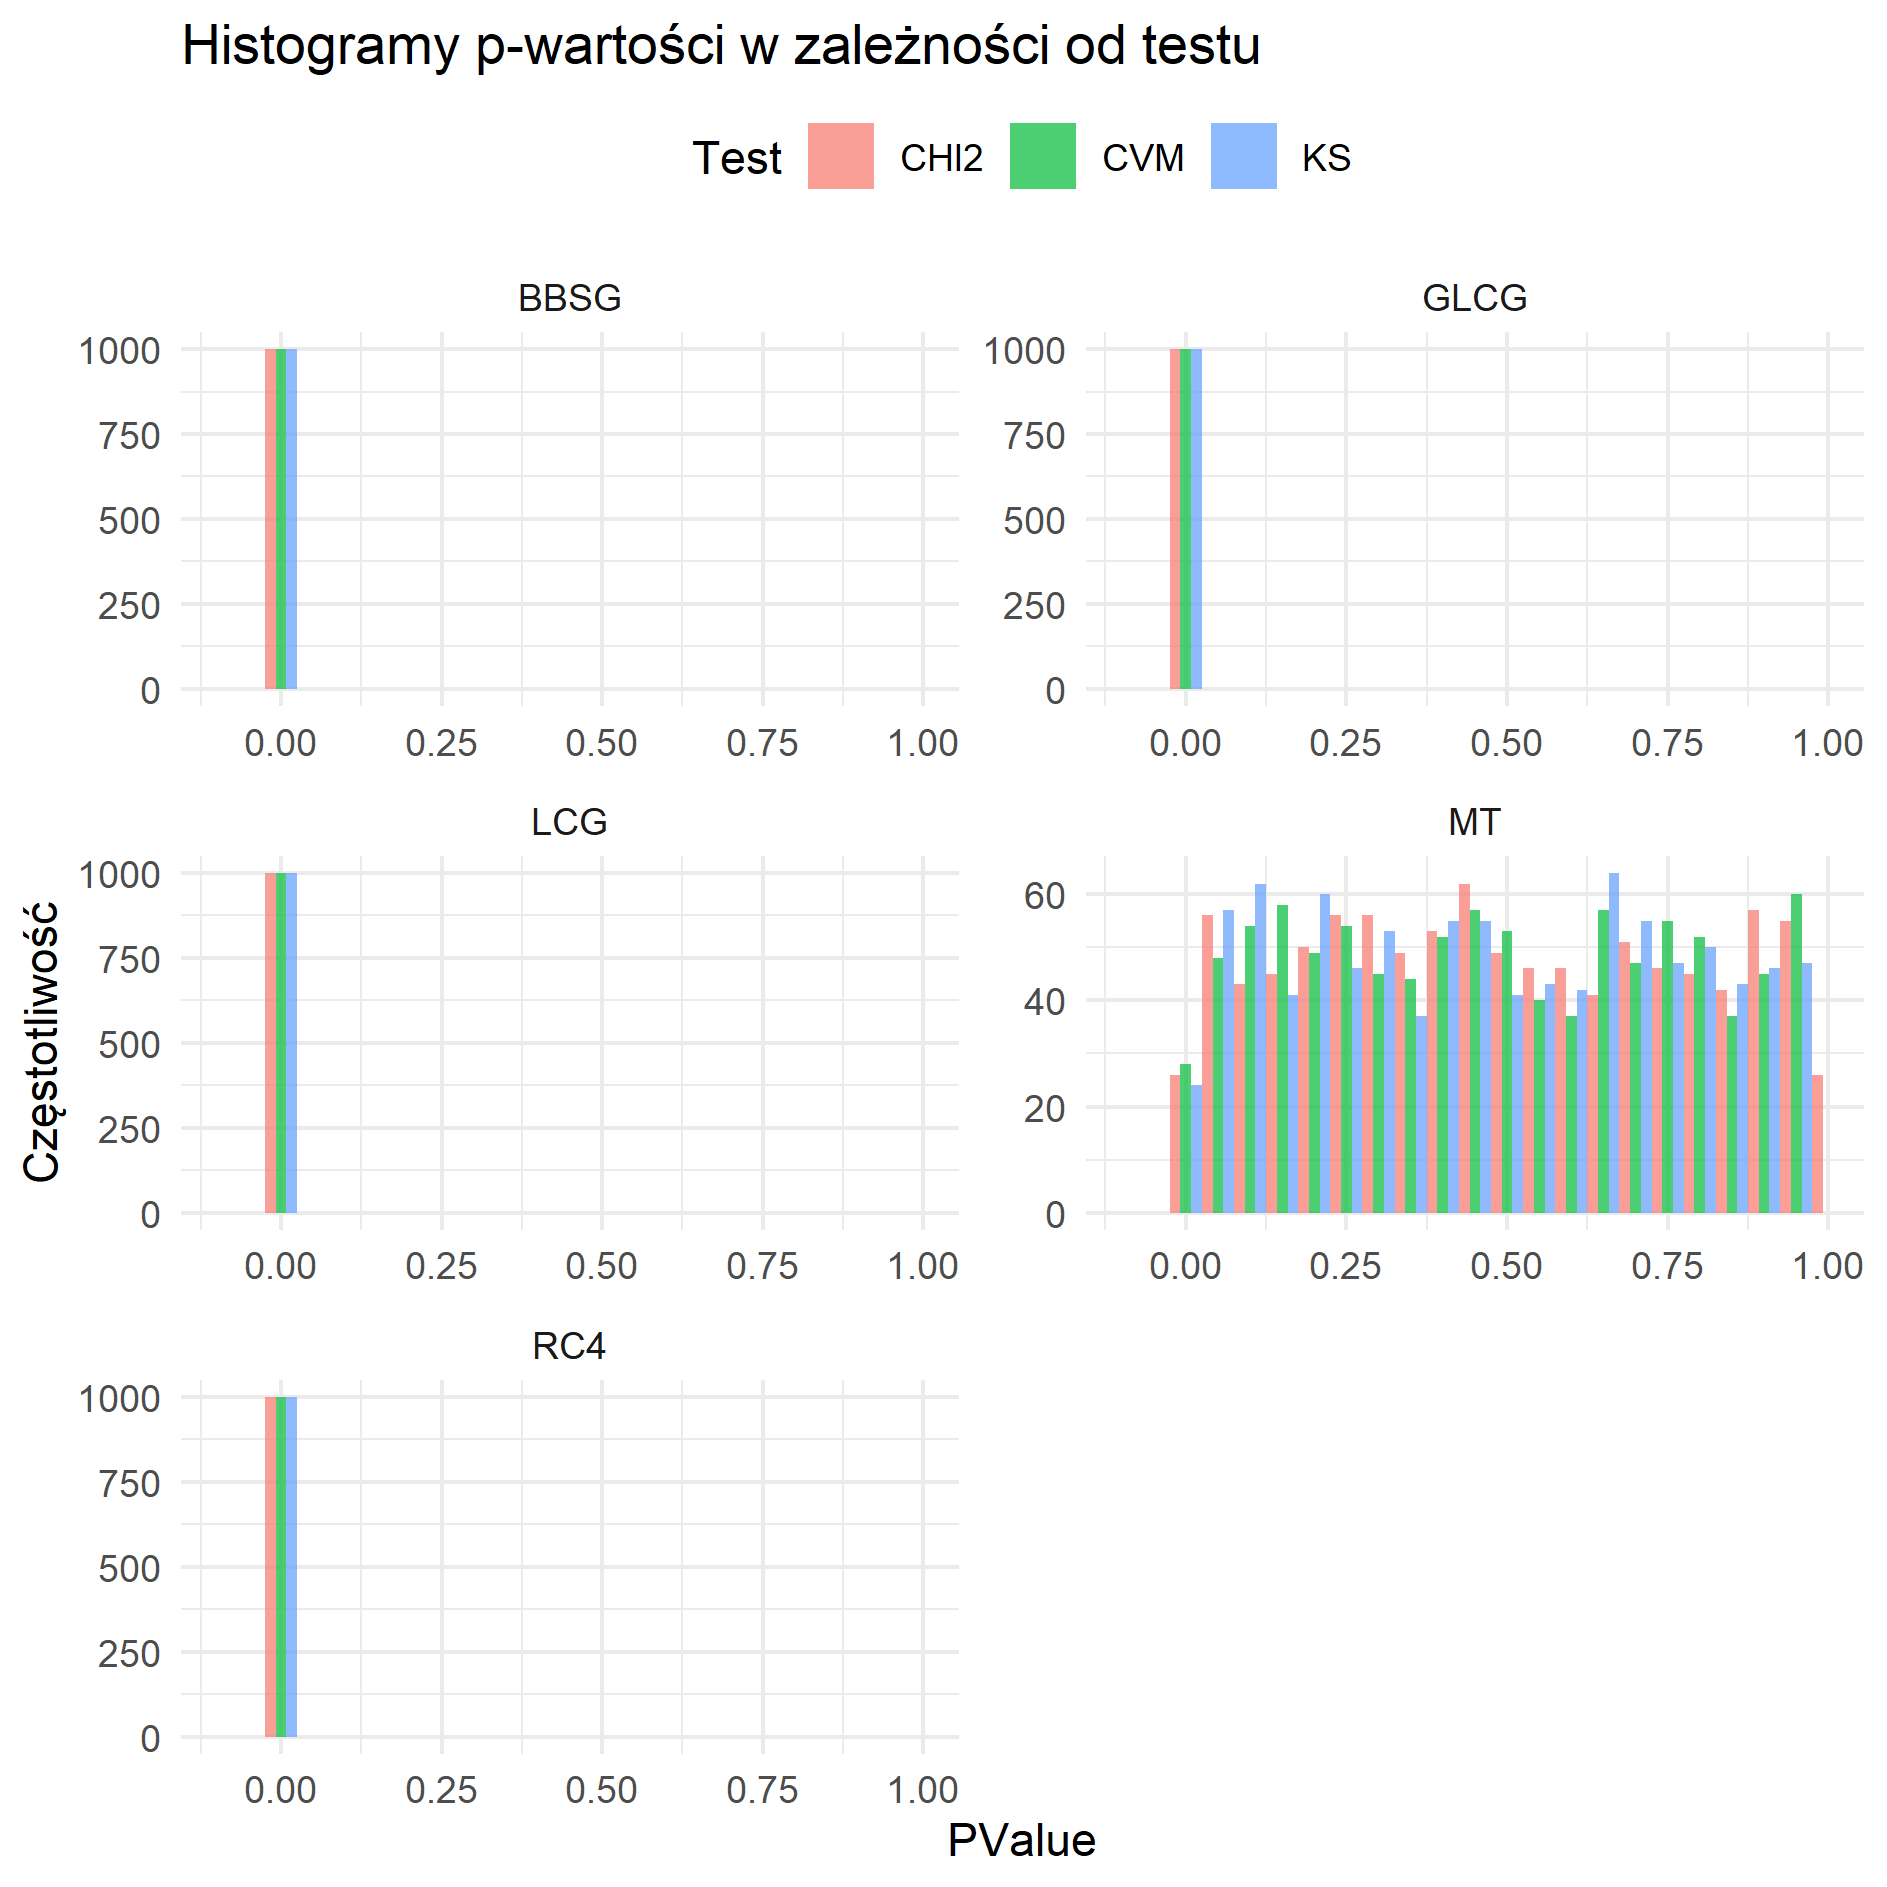
\includegraphics[scale=0.7]{p_wartosc_a_test_2.png}
\caption{\newline Wyk.2 Rozkład p wartości testów dla  wygenerowanych ciagów liczb długości $2^{15}$}
\end{center}

O ile zwiększenie ilości generowanych liczb nie wpłynęło bardzo wykres generatora Mersenne Twistera, to w pozostałych generatorach p$\_$wartości są już bardzo bliskie 0. Wpływ na to może mieć np to, że okres naszych generatorów jest mniejszy od ilości stworzonych liczb.

Spojrzyjmy jeszcze na wyniki second-level testing.

\begin{table}[h!]
\centering
\begin{tabular}{|c|c|c|c|c|c|}
\hline
 & RC4 & LCG & GLCG & BBSG & MT \\ \hline
CHI2 & 0.0 & 0.0 & 0.0 & 0.0 & 0.67 \\ \hline
KS & 0.0 & 0.0 & 0.0 & 0.0 & 0.47 \\ \hline
CVM & 0.0 & 0.0 & 0.0 & 0.0 & 0.35 \\ \hline
\end{tabular}
\caption{Wyniki second-level testing dla wybranych generatorów.}
\label{tab:zero_table}
\end{table}

Jak widzimy, nasze przypuszczenia się potwierdziły. Najlepszym generatorem liczb pseudolosowych spośród wszyskich generatorów wybranych przez nas jest generator Mersenne Twistera. Pozostałe generatory dały wyniki zerowe. 

W drugiej części zadania sprawdzaliśmy czy liczby $\pi$, $e$, $\sqrt{2}$ mogą posłużyć nam jako generatory liczb. Wykorzystując frequency monobit test oraz binarny zapis tych liczb(milionowe rozwinięcie) otrzymaliśmy wyniki p$\_$wartości:


\begin{table}[h!]
\centering
\begin{tabular}{|c|c|}
\hline
liczba - generator & p$\_$wartość \\ \hline
\pi & 0.6137 \\ \hline
$e$ & 0.9269  \\ \hline
$\sqrt{2}$ & 0.8177 \\ \hline
\end{tabular}
\caption{Wyniki frequency monobit test dla  trzech liczb niewymiernych.}
\end{table}

Wszystkie trzy liczby jako generatory dają po stestowaniu zadowalający wynik. Jednak warto zauważyć, że są to liczby wykorzystujące 1 000 000 miejsc w zapisie binarnym.
W celu przeprowadzenia second-level testing dla tych liczb, musimy ich zapis binarny podzielić na mniejsze części. 

\begin{center}
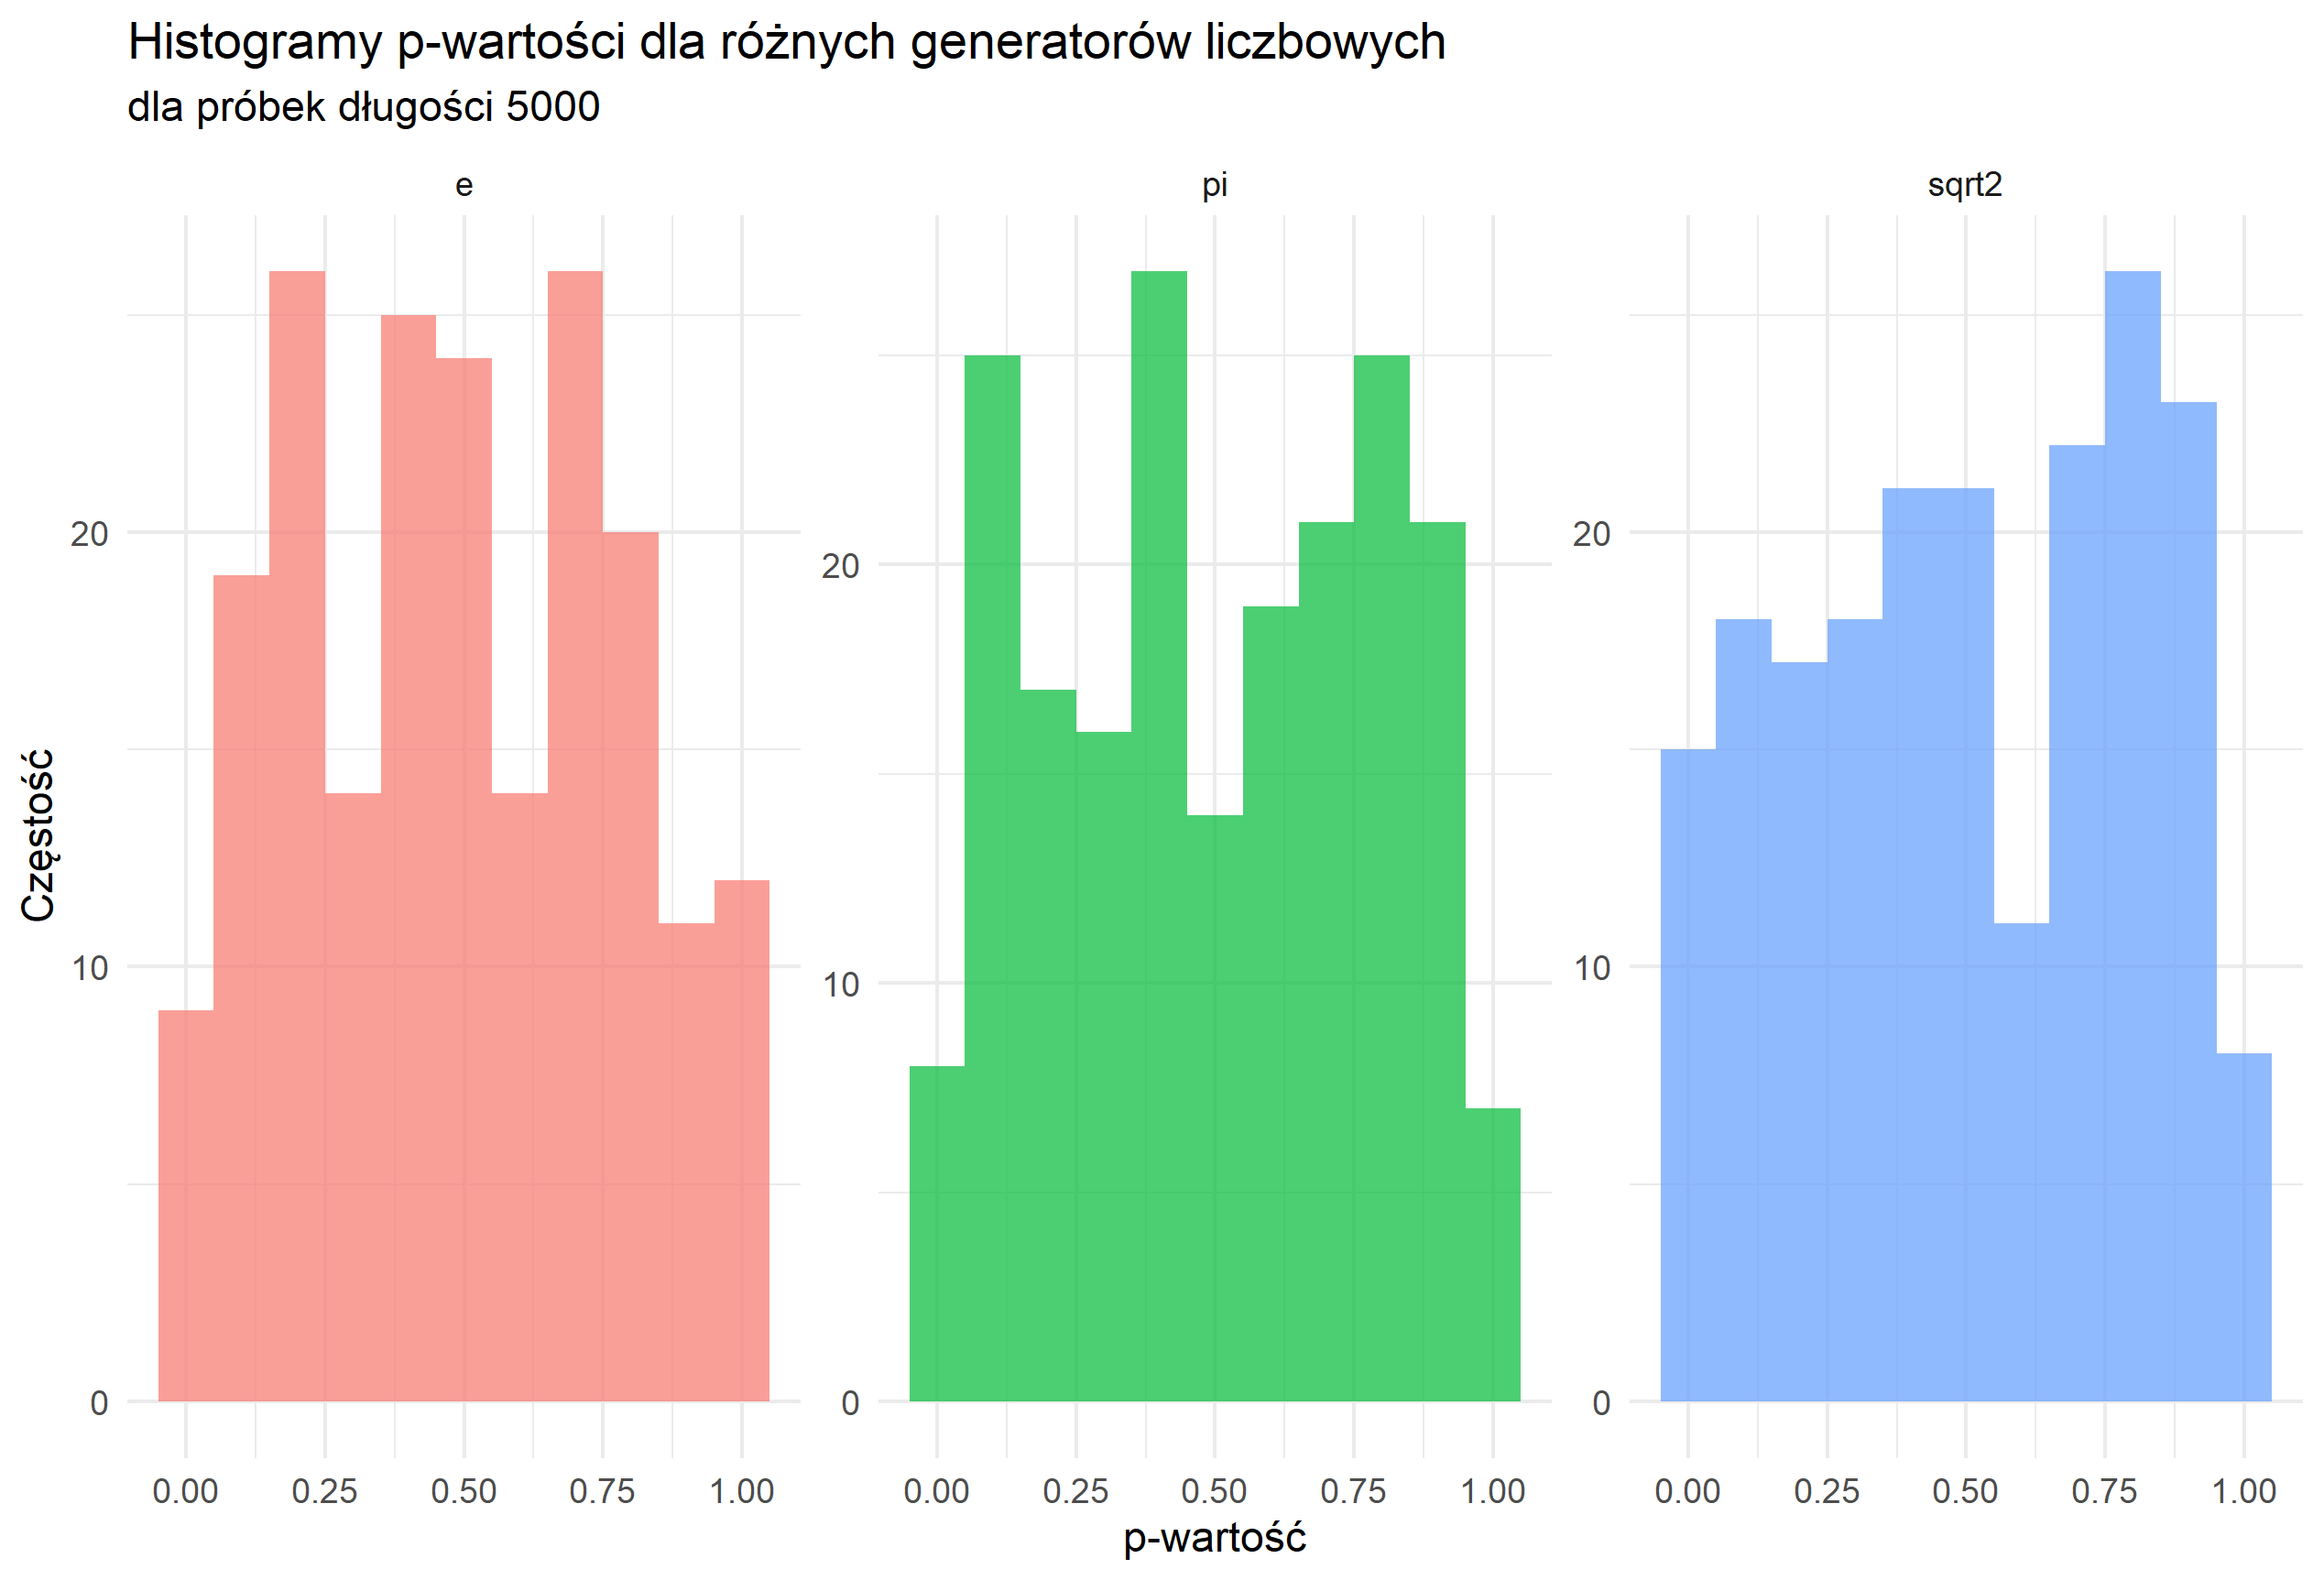
\includegraphics[scale=0.7]{p_liczby_5000.png}
\caption{Wyk.3 Rozkład p wartości dla fragmentów liczb niewymiernych jako generatorów w frequency monobit test}
\end{center}

Powyżej widzimy wyniki p$\_$wartości dla frequency monobit test obliczanych dla próbek długości 5000. Ich rozkład nie jest idealnie jednostajny, jednak możemy przypuszczać, że generatory tej długości są dobrym wyborem w celu tworzenia liczb pseudolosowych. Porównamy jednak jeszcze wyniki second-level testing dla  różnej długości próbki generatora.

\begin{table}[h!]
\centering
\begin{tabular}{|c|c|c|c|}
\hline
 & n = 10 000 & n = 5 000 & n = 1 000\\ \hline
\pi & 0.2622 & 0.7399 & 0.0\\ \hline
$e$ & 0.2757 & 0.6890 & 0.0 \\ \hline
$\sqrt{2}$ & 0.3669 & 0.6215 & 0.0\\ \hline
\end{tabular}
\caption{P$\_$wartości dla second-level testing dla trzech liczb niewymiernych.}
\end{table}

W powyższej tabeli $n$ oznacza jaką długość miały nasze generatory stworzone z części zapisu tych liczb wymiernych. Widzimy, że generatory długości 5 000 były już wystarczające aby tworzyć dobre pseudolosowe liczby, natomiast $n$=1000 było za krótką długością.
\newpage
\section*{Odnośnik do kodu}

\begin{table}[h!]
\centering
\begin{tabular}{|c|p{6cm}|p{6cm}|}
\hline
\textbf{Obiekt} & \textbf{Kod w Pythonie} & \textbf{Kod w R} \\ \hline
Wyk. 1, Wyk.2 & generate$\_$and$\_$test$\_$generators() - funkcja wykorzystana do tworzenia wyników & read$\_$pvalues - funkcja do wczytania danych, \newline
p$\_$wartosi$\_$wykres - zmienna zawierająca tworzony wykres
\\ \hline
Wyk. 3 & monobit$\_$fragmenty(5000) - zapisanie p$\_$wartości, przeprowadzenie second-level testing & p$\_$values$\_$data5000 - wczytana ramka danych, \newline
liczby$\_$5000 - zmienna zawierająca tworzony wykres \\ \hline
Tabela 1 & generate$\_$and$\_$test$\_$generators() - funkcja wykorzystana do tworzenia wyników & - \\ \hline
Tabela 2 & frequency$\_$monobit$\_$test() - funkcja wykorzystana do tworzenia wyników,\newline
wyświetlenie wyników - pod komentarzem: monobit na digits$\_$number & - \\ \hline
Tabela 3 & monobit$\_$fragmenty() - funkcja gdzie zmienną są długość podziałów liczb &  - \\ \hline
\end{tabular}

\end{table}

\end{document}
